
\chapter{Data Preprocessing}
\label{chapter:data-preprocessing}
To successfully extract the characteristics of the sample populations in an article, which includes the experimental stage, the ethnicity groups of individuals involved and the size of sample population pool, it is necessary to obtain the text data of the article and prepare it for further processing and information extraction task. This information extraction.task involves steps like converting PDF documents to XML files, extracting textural information from XML file, recognition of suitable candidates for entities and transforming words into vectors using pre-trained embeddings. This chapter describes the preprocessing steps required to make sure that the source documents are ready for relation extraction using neural networks. 

\section{PDF to XML Conversion}
\label{section:pdf-to-xml-conversion}
Majority of the published scientific literature available today is in form of PDF documents with little or no free text associated with them. The PDF standard does not attempt to encode any semantic connection between the characters in a word or between paragraphs which makes the ease of extracting text an orthogonal issue to the file format. As such, the researchers wanting to do text mining on a large number of journals need to transcribe the PDF documents to text based formats like plain text, XMLs or HTMLs. To overcome this, we used an in-house document conversion pipeline \cite{Goyal2016712} to extract textual information from PDF files and convert them to XML documents using different tools and platforms. 

\begin{figure}[!ht]
    \centering
    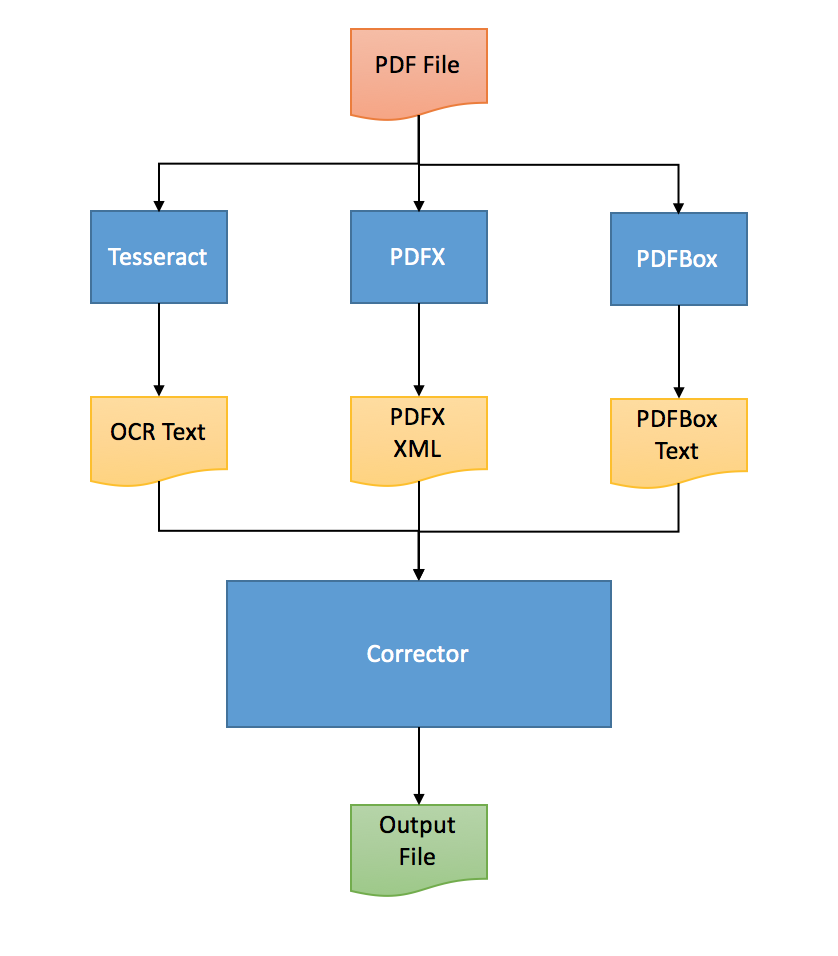
\includegraphics[height=0.55\textheight]{Images/BioPDFx-Flowchart.png}
    \caption{Flowchart diagram for PDF to XML conversion pipeline showing different text extraction modules followed by a corrector stage}
    \label{figure:biopdfx-flowchart}
    \vspace{0.1in}
\end{figure}

An overview of the pipeline is depicted in Figure \ref{figure:biopdfx-flowchart}. In this workflow, we provide each PDF file to three different modules which run independently in parallel and extract text from PDF files using various extraction tools. PDFX is a web-service designed to reconstruct the logical structure of scholarly articles in PDF form and output them as an XML document. The final XML document depicts the input article's logical structure in terms of title, sections, tables, references, etc. and also links it to geometrical typesetting markers in the original PDF document, such as paragraph and column breaks. PDFBox is an open-source Java library which we are using to extract textual information from a PDF file and then using it for further processing. As a final step of text extraction, we use Tesseract which is a raw OCR tool with high character recognition accuracy and extracts text in a simple textual format without any formatting.

Using the outputs from the above three modules, we run the corrector stage, which manipulates and combines them to produce the final output. The corrector stage is a combination of multiple correctors where each corrector acts on the output from the previous one in a serialized manner. Various correctors that are run as a part of this stage perform the {\it Abstract Tile correction}, {\it Special Character correction} and {\it Reference Acknowledgement corrections} to produce an output in XML format. These correctors improve the overall quality of the final output file and remove the unwanted sections like metadata, etc. from the perspective of information extraction. The final XML file contains section-wise text according to source PDF file which is perfect for further text mining activities. 

\section{XML to Text Transcription}
\label{section:xml-to-text-transcription}
The full text of the articles to be used for relation extraction is obtained by traversing these XML files created through above PDF transcription engine. Some XML files were also collected as publicly-available NXMLs from PubMed Central, a free full-text archive of biomedical and life science literature. When traversing these XML files, text from several tags was ignored entirely as the content from those labels was known to be irrelevant to the task of extraction of population characteristics. These tags contained either metadata information related to the publication and not the actual content or were formatting tags for specifying the design of the article. A total of 22 such tags were identified and used for removal during extraction of text from the article. These fell into various categories like article metadata which included {\it article-id}, {\it journal-meta}, {\it copyright-statement}, etc. or formatting tags like {\it fpage}, {\it lpage} or other irrelevant tags.

The text obtained from the XMLs was further parsed to remove the elements that are less relevant to the task and clean the remaining text to make extraction simpler. Regular expression-based preprocessing is primarily geared at removing irrelevant or extraneous numbers that might lead to false positives for sample sizes, as well as normalizing the representations of numbers that may give rise to the correct values being missed. A total of 23 such patterns were parsed and removed or rewritten using regular expressions. Some of the examples include:

\begin{itemize}
    \item \emph{Removal of commas}: 
    Commas that mark the thousandth, etc. digits of a number are removed. For example, ``$12,696$'' becomes ``$12696$''
    
    \item \emph{Mathematical or scientific notation}:
    Numbers that can be inferred to be irrelevant to sample size extraction based on the surrounding context are removed, such as ``$p=8.14 \times 10^{-05}$'', ``$3 \log 10$''.

    \item \emph{In-line references}:
    References within the text to other publications or elements within the same article are removed, such as ``[10, 21]'' and ``Fig. 12''.

    \item \emph{Units and elements}:
    Descriptions of units or known elements are removed from the text, such as ``1,020 SNPs'', ``23 mg/L''
\end{itemize}

\section{Entity Detection}
\label{section:entity-detection}
Once the source article is transcribed to plain text and is ready for the extraction of relevant information, we need to identify passages that may contain information related to the population characteristics. This task of passage identification should be inclusive in the sense that any candidate passage will be extracted and no relevant passage would be omitted. The identification of passages is primarily made by recognizing the entity mentions in the text potentially corresponding either to the ethnicity values or a sample size value (described in detail below) and extracting their surrounding passages. This task is particularly important for our case as we need to match the entries in the curated database with real mentions in the text which are not always exact string matches or even exact synonyms.

After identification of the passages, we need to detect the candidates for ethnicity groups of genome-wide association studies' populations, the size of the population involved and stage of the survey which would serve as the base for the relation extraction tasks. This operation is not required in case of annotated text where the candidate entities are already tagged using different crowd-sourcing methods as discussed in previous sections. However, in our case, where we are using entries from the curated database as training examples for our system, we need to correctly identify these entities by matching them from curated entries to mentions in the text. These selection criteria and entity preparation are achieved by studying the properties associated with these objects and also using the ``extraction guideline'' \cite{hindorff2014catalog} as provided by the curation teams NHGRI and EBI.  The process of identification of these candidate entities was completed under collaborative work \cite{kashyapthesis} and is discussed below:

\begin{itemize}
    \item \emph{Ethnicity}:
    We constructed the dictionary of ethnicity mappings using a multitude of terms that can refer to the ethnicity of an individual, including the country of origin (e.g. ``Germany''), the specific ethnicity group (e.g. ``European''), an adjectival for the country (e.g. ``German'') and similar sets of terms for cities and other regions with this knowledge being based on the CIA World Factbook \footnote{CIA World Factbook: \url{http://www.cia.gov/library/publications/the-world-factbook}}. The final dictionary comprises 449 terms that map to 14 top-level ethnicity groups which cover a majority of the mentions in text.
    
    \item \emph{Sample Size}:
    A typical GWAS article may contain hundreds of numeric values and considering each instance of a numeric value a potential candidate for sample size leads to a huge increase in the number of false positives which renders the dictionary tagging approach ineffective.  We therefore use a Conditional Random Field model to tag instances of numeric values in text that appear to correspond an experimental sample based on multiple syntactic and semantic features of the surrounding textual content. The output of the CRF tagger was a set of tokens in text which was most likely to correspond to the sizes of the experimental samples in the GWAS.
    
    \item \emph{Stage}:
    A rule-based classifier was modified for identification of stage entities to use the presence of stage-specific words to make its prediction (e.g., ``discovery'' or ``first stage'' for the initial stage, or ``follow-up'' or ``second stage'' for replication). These classifier was used to tag different tokens in the input text as a candidate for the stage mentions in the relationship tuples.
 \end{itemize}

\section{Word Representation}
\label{section:word-embeddings}
After detecting entity pairs for relation mentions in the text, we need to encode the text in a form which is easily understandable by neural networks. This encoding is required because convolutional neural networks were originally developed for image data which is fixed-sized, low-dimensional and dense whereas text documents are variable-sized, high-dimensional and sparse if represented by a sequence of one-hot vectors. Therefore, in most of CNN studies on text, the words in sentences are first converted to low-dimensional word vectors which are often obtained by some other method similar to language modeling from an additional large corpus. We are using {\it word2vec} \cite{mikolov2013distributed} tool which is a two-layer neural network model to produce word embeddings according to their linguistic context. The word embeddings created using word2vec can capture different degrees of similarity between the phrase and various semantic, and syntactic patterns can be reproduced using vector arithmetic. For this thesis, we are using word vectors that were induced using the {\it word2vec} tool from over 5.5 Billion tokens which were derived using a combination of all the abstracts from the PubMed publications and all the full-text documents from the PubMed Central Open Access subset. These literature sources effectively cover the entire available biomedical domain scientific research and are a useful resource for this area of study.

Apart from word embeddings, we also need a way to encode the entity candidates for the relation mentions in the text. Apparently, it is not possible to capture the structural information (like shortest dependency path between the entity pairs) only through word embeddings. For this purpose, we also use position embeddings in the case of relation extraction problems. A positional embedding can be defined as the combination of the relative distances of the current word to each of the candidate entities $e_1$ and $e_2$.  For each word, we define the relative distance between the word and a candidate entity as the number of words between them and are represented using a vector of dimensionality two which, therefore, creates a positional embedding for each word a vector of size 4. A sample raw sentence with marked entities and its transformation into vector encoding using both word and positional embeddings is depicted in Figure \ref{figure:embeddings-example}

\vspace{0.1in}
\begin{figure}[ht]
    \centering
    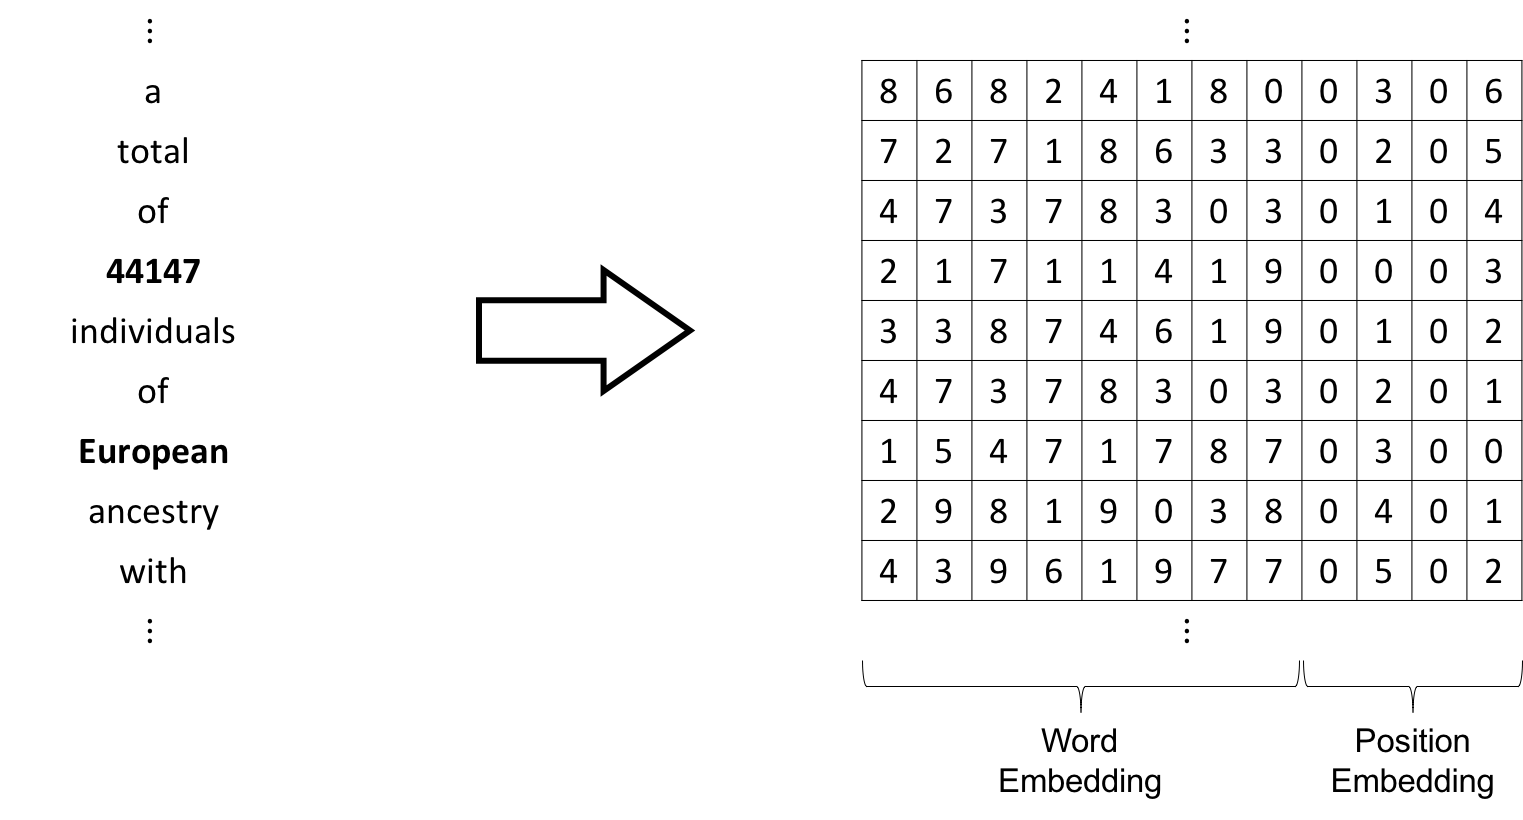
\includegraphics[width=0.85\linewidth]{Images/Embeddings-Example.png}
    \caption{Example input text snippet with its transformation into a matrix representation using word and position embeddings}
    \label{figure:embeddings-example}
\end{figure}

The work in Section \ref{section:pdf-to-xml-conversion} is a reprint of the material as it appears in ``Natural Language Processing using Kepler Workflow System: First Steps'' in Procedia Computer Science, Vol. 80. I am thankful to my co-authors Alok Singh, Shitij Bhargava, Daniel Crawl, Ilkay Altintas, and Chun-Nan Hsu for their inputs and support during the research work. The thesis author was the primary investigator and author of this paper.  

Material from Chapter \ref{chapter:data-preprocessing} in part is currently being prepared for submission for the publication of material. The thesis author was the primary investigator and author of this material.